% soliton cheat sheet: two landscape A4 pages.  Build: make cheatsheet
% Every number here comes from lib/soliton_ctl.h, lib/soliton_field.h and
% lib/soliton_voice.h (dial values and speeds printed from that code).
\documentclass{article}
\usepackage[a4paper,landscape,margin=6mm]{geometry}
\usepackage[T1]{fontenc}
\usepackage{lmodern}
\usepackage[default]{sourcesanspro}
\usepackage{amssymb}
\usepackage{amsmath}
\usepackage{tikz}
\usepackage[most]{tcolorbox}
\usepackage{array}
\usepackage{tabularx}
\pagestyle{empty}
\setlength{\parindent}{0pt}

\definecolor{ink}{RGB}{30,30,30}
\definecolor{snd}{RGB}{20,20,20}       % SOUND-page knob labels
\definecolor{fdc}{RGB}{0,130,120}      % FIELD-page knob labels
\definecolor{fxc}{RGB}{30,90,170}      % FX-page knob labels
\definecolor{ampc}{RGB}{67,160,71}     % amp envelope
\definecolor{modc}{RGB}{230,140,20}    % mod envelope
\definecolor{lfoc}{RGB}{150,60,170}    % LFO
\definecolor{fltc}{RGB}{215,60,50}     % filter
\definecolor{engc}{RGB}{190,40,110}    % engine parameters
\definecolor{freec}{RGB}{170,170,170}  % unassigned
\definecolor{padc}{RGB}{120,170,230}

\newcommand{\FX}[1]{\textcolor{fxc}{#1}}
\newcommand{\FD}[1]{\textcolor{fdc}{#1}}
\newcommand{\EN}[1]{\textcolor{engc}{#1}}
\newcommand{\FR}[1]{\textcolor{freec}{#1}}
\newcommand{\cc}[1]{\textcolor{black!45}{\fontsize{4.6}{5}\selectfont #1}}

% knob: x, SOUND label (above), FIELD label, FX label (below)
\newcommand{\knob}[4]{%
  \draw[fill=black!8, draw=black!60, line width=0.4pt] (#1,63) circle (3.4);
  \draw[black!60, line width=0.5pt] (#1,63) -- ++(110:2.9);
  \node[font=\fontsize{5.6}{6.2}\selectfont\bfseries, text=snd, align=center] at (#1,70.2) {#2};
  \node[font=\fontsize{5.4}{6}\selectfont\bfseries, text=fdc, align=center] at (#1,56.4) {#3};
  \node[font=\fontsize{5.4}{6}\selectfont, text=fxc, align=center] at (#1,52.4) {#4};}
% pad: col (0..7), row (1 top, 0 bottom), label
\newcommand{\pad}[3]{%
  \draw[rounded corners=0.8mm, fill=padc!35!white, draw=padc!80!black, line width=0.4pt]
    (36+#1*13.2, 21+#2*13.2) rectangle ++(12,12);
  \node[font=\fontsize{5.4}{6}\selectfont, text=ink, align=center, text width=11mm]
    at (36+#1*13.2+6, 21+#2*13.2+6) {#3};}
% fader: x, top label, colour
\newcommand{\fader}[3]{%
  \draw[fill=black!12, draw=black!50] (#1-0.7,26) rectangle (#1+0.7,52);
  \draw[fill=#3!60!white, draw=#3!70!black, rounded corners=0.4mm] (#1-2.6,36) rectangle (#1+2.6,40);
  \node[font=\fontsize{5.6}{6.2}\selectfont\bfseries, text=#3!70!black, align=center] at (#1,56) {#2};}
% small button: x, y, label, colour, width
\newcommand{\btn}[5]{%
  \draw[rounded corners=0.6mm, fill=#4!25!white, draw=#4!70!black, line width=0.4pt]
    (#1-#5/2,#2-2.6) rectangle (#1+#5/2,#2+2.6);
  \node[font=\fontsize{4.9}{5.4}\selectfont, text=ink, align=center] at (#1,#2) {#3};}

\tcbset{card/.style={enhanced, colback=white, colframe=black!70, boxrule=0.5pt, arc=1.5mm,
    left=1.6mm, right=1.6mm, top=1.1mm, bottom=1.1mm, toptitle=0.6mm, bottomtitle=0.6mm,
    fonttitle=\bfseries\fontsize{8.6}{10}\selectfont, coltitle=white, colbacktitle=black!75,
    fontupper=\fontsize{7.1}{8.5}\selectfont, before skip=0mm, after skip=1.8mm}}
\newtcolorbox{card}[1]{card, title={#1}}
\newcolumntype{L}{>{\raggedright\arraybackslash}X}

\begin{document}

{\fontsize{16}{18}\selectfont\bfseries soliton}\hspace{3mm}%
{\fontsize{9.5}{11}\selectfont Axoloti Core + Launchkey 49 MK3 (standalone mode) \textperiodcentered{}
3 voices, each a field under a nonlinear PDE \textperiodcentered{} \texttt{patches/soliton/soliton\_v1.axp}}\hfill
{\fontsize{7}{8}\selectfont\color{black!55} v1.0 \textperiodcentered{} 2026-11-12 \textperiodcentered{} page 1 of 2 \textperiodcentered{} github.com/ndlopes-github/axoloti-playground}

\vspace{1.5mm}
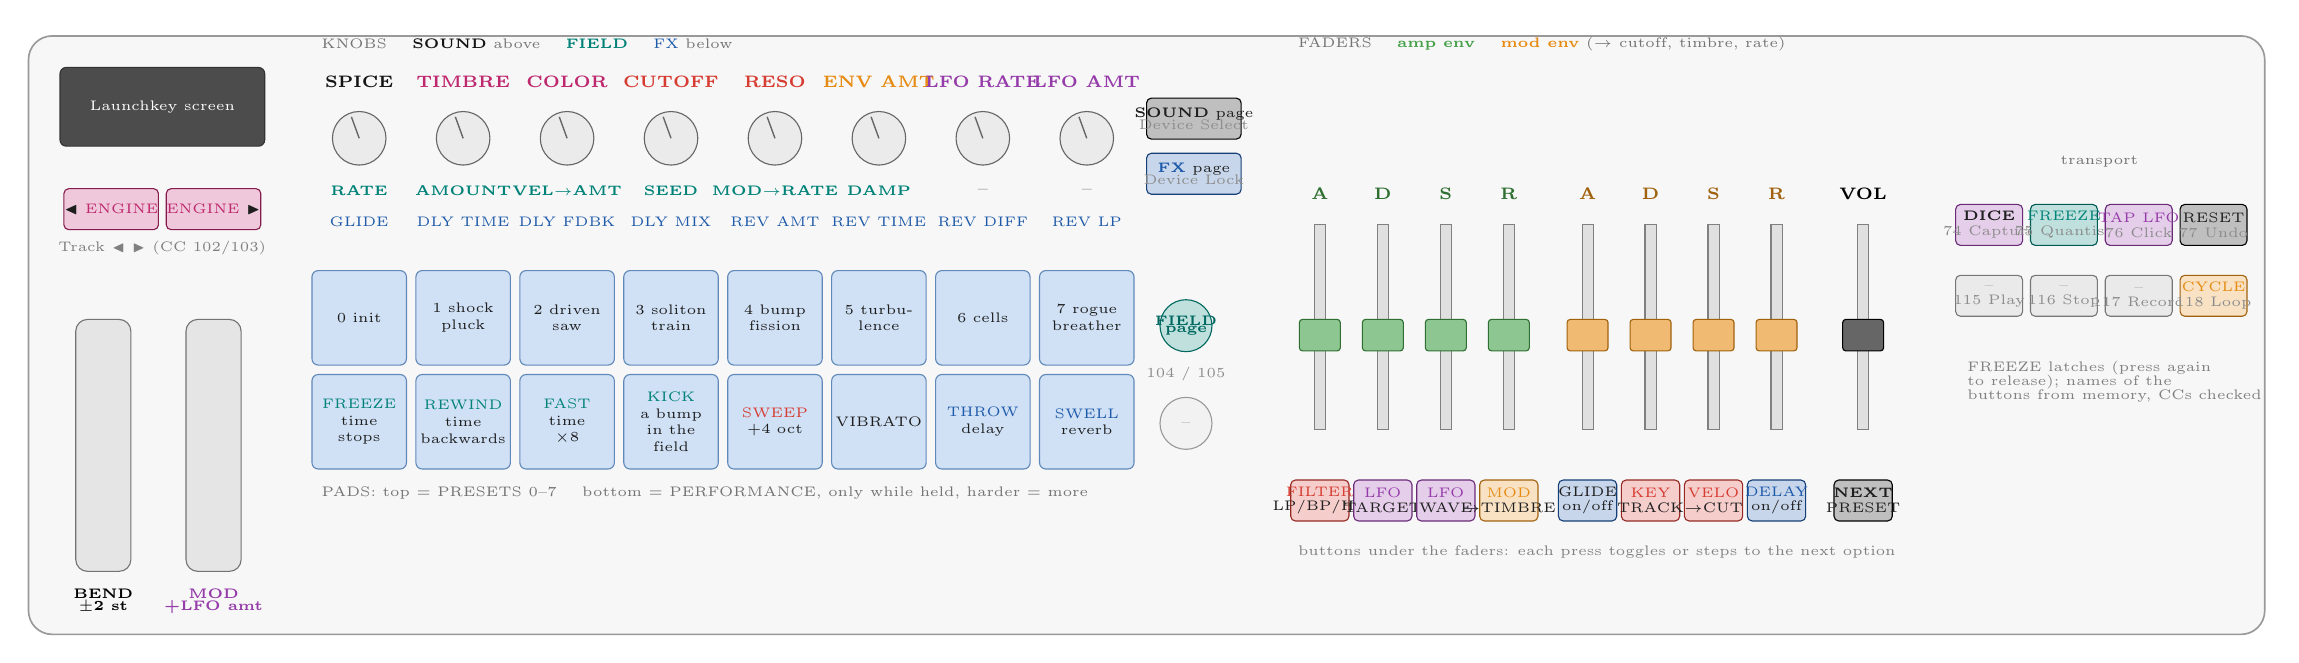
\begin{tikzpicture}[x=1mm,y=1mm]
  \draw[rounded corners=3mm, fill=black!3, draw=black!40, line width=0.6pt] (0,0) rectangle (284,76);

  % ---- left: screen, track buttons, wheels
  \draw[fill=black!70, draw=black!80, rounded corners=0.8mm] (4,62) rectangle (30,72);
  \node[font=\fontsize{5}{6}\selectfont, text=white] at (17,67) {Launchkey screen};
  \btn{10.5}{54}{\(\blacktriangleleft\) \EN{ENGINE}}{engc}{12}
  \btn{23.5}{54}{\EN{ENGINE} \(\blacktriangleright\)}{engc}{12}
  \node[font=\fontsize{4.6}{5}\selectfont, text=black!50] at (17,49) {Track \(\blacktriangleleft\) \(\blacktriangleright\) (CC 102/103)};
  \draw[rounded corners=1.5mm, fill=black!10, draw=black!55] (6,8) rectangle (13,40);
  \draw[rounded corners=1.5mm, fill=black!10, draw=black!55] (20,8) rectangle (27,40);
  \node[font=\fontsize{5.4}{6}\selectfont\bfseries, align=center] at (9.5,4.2) {BEND\\[-0.6mm]\(\pm\)2 st};
  \node[font=\fontsize{5.4}{6}\selectfont\bfseries, align=center, text=lfoc] at (23.5,4.2) {MOD\\[-0.6mm]+LFO amt};

  % ---- knobs: SOUND (black, top) / FIELD (green) / FX (blue)
  \node[font=\fontsize{5}{6}\selectfont, text=black!55, anchor=west] at (36,75) {KNOBS \quad
     \textbf{\textcolor{snd}{SOUND}} above \quad \textbf{\FD{FIELD}} \quad \FX{FX} below};
  \knob{42}{SPICE}{\FD{RATE}}{\FX{GLIDE}}
  \knob{55.2}{\EN{TIMBRE}}{\FD{AMOUNT}}{\FX{DLY TIME}}
  \knob{68.4}{\EN{COLOR}}{\FD{VEL\(\to\)AMT}}{\FX{DLY FDBK}}
  \knob{81.6}{\textcolor{fltc}{CUTOFF}}{\FD{SEED}}{\FX{DLY MIX}}
  \knob{94.8}{\textcolor{fltc}{RESO}}{\FD{MOD\(\to\)RATE}}{\FX{REV AMT}}
  \knob{108}{\textcolor{modc}{ENV AMT}}{\FD{DAMP}}{\FX{REV TIME}}
  \knob{121.2}{\textcolor{lfoc}{LFO RATE}}{\FR{--}}{\FX{REV DIFF}}
  \knob{134.4}{\textcolor{lfoc}{LFO AMT}}{\FR{--}}{\FX{REV LP}}
  \btn{148}{65.5}{\textbf{SOUND} page\\[-0.4mm]\cc{Device Select}}{black}{12}
  \btn{148}{58.5}{\textbf{\FX{FX}} page\\[-0.4mm]\cc{Device Lock}}{fxc}{12}

  % ---- pads + round buttons
  \pad{0}{1}{0 init} \pad{1}{1}{1 shock\\pluck} \pad{2}{1}{2 driven\\saw} \pad{3}{1}{3 soliton\\train}
  \pad{4}{1}{4 bump\\fission} \pad{5}{1}{5 turbu-\\lence} \pad{6}{1}{6 cells} \pad{7}{1}{7 rogue\\breather}
  \pad{0}{0}{\FD{FREEZE}\\time\\stops} \pad{1}{0}{\FD{REWIND}\\time\\backwards} \pad{2}{0}{\FD{FAST}\\time\\\(\times\)8} \pad{3}{0}{\FD{KICK}\\a bump\\in the field}
  \pad{4}{0}{\textcolor{fltc}{SWEEP}\\+4 oct} \pad{5}{0}{VIBRATO} \pad{6}{0}{\FX{THROW}\\delay} \pad{7}{0}{\FX{SWELL}\\reverb}
  \node[font=\fontsize{5}{6}\selectfont, text=black!55, anchor=west] at (36,18) {PADS: top = PRESETS 0--7 \quad bottom = PERFORMANCE, only while held, harder = more};
  \draw[fill=fdc!25!white, draw=fdc!80!black] (147,39.2) circle (3.3);
  \draw[fill=black!5, draw=black!40] (147,26.8) circle (3.3);
  \node[font=\fontsize{4.6}{5}\selectfont\bfseries, align=center, text=fdc!80!black] at (147,39.2) {FIELD\\[-0.8mm]page};
  \node[font=\fontsize{4.6}{5}\selectfont, align=center, text=freec] at (147,26.8) {--};
  \node[font=\fontsize{4.2}{5}\selectfont, text=black!45] at (147,33) {104 / 105};

  % ---- faders
  \node[font=\fontsize{5}{6}\selectfont, text=black!55, anchor=west] at (160,75) {FADERS \quad
     \textcolor{ampc}{\textbf{amp env}} \quad \textcolor{modc}{\textbf{mod env}} (\(\to\) cutoff, timbre, rate)};
  \fader{164}{A}{ampc} \fader{172}{D}{ampc} \fader{180}{S}{ampc} \fader{188}{R}{ampc}
  \fader{198}{A}{modc} \fader{206}{D}{modc} \fader{214}{S}{modc} \fader{222}{R}{modc}
  \fader{233}{VOL}{black}
  \btn{164}{17}{\textcolor{fltc}{FILTER}\\LP/BP/HP}{fltc}{7.4}
  \btn{172}{17}{\textcolor{lfoc}{LFO}\\TARGET}{lfoc}{7.4}
  \btn{180}{17}{\textcolor{lfoc}{LFO}\\WAVE}{lfoc}{7.4}
  \btn{188}{17}{\textcolor{modc}{MOD}\\\(\to\)TIMBRE}{modc}{7.4}
  \btn{198}{17}{GLIDE\\on/off}{fxc}{7.4}
  \btn{206}{17}{\textcolor{fltc}{KEY}\\TRACK}{fltc}{7.4}
  \btn{214}{17}{\textcolor{fltc}{VELO}\\\(\to\)CUT}{fltc}{7.4}
  \btn{222}{17}{\FX{DELAY}\\on/off}{fxc}{7.4}
  \btn{233}{17}{\textbf{NEXT}\\PRESET}{black}{7.4}
  \node[font=\fontsize{4.6}{5}\selectfont, text=black!50, anchor=west] at (160,10.5) {buttons under the faders: each press toggles or steps to the next option};

  % ---- transport (ch 16)
  \node[font=\fontsize{5}{6}\selectfont, text=black!55] at (263,60) {transport};
  \btn{249}{52}{\textbf{DICE}\\\cc{74 Capture}}{lfoc}{8.5}
  \btn{258.5}{52}{\FD{FREEZE}\\\cc{75 Quantise}}{fdc}{8.5}
  \btn{268}{52}{\textcolor{lfoc}{TAP LFO}\\\cc{76 Click}}{lfoc}{8.5}
  \btn{277.5}{52}{RESET\\\cc{77 Undo}}{black}{8.5}
  \btn{249}{43}{\FR{--}\\\cc{115 Play}}{freec}{8.5}
  \btn{258.5}{43}{\FR{--}\\\cc{116 Stop}}{freec}{8.5}
  \btn{268}{43}{\FR{--}\\\cc{117 Record}}{freec}{8.5}
  \btn{277.5}{43}{\textcolor{modc}{CYCLE}\\\cc{118 Loop}}{modc}{8.5}
  \node[font=\fontsize{4.6}{5.2}\selectfont, text=black!50, align=left, anchor=north west] at (245,36)
     {FREEZE latches (press again\\to release); names of the\\buttons from memory, CCs checked};
\end{tikzpicture}

\vspace{1.2mm}
\begin{minipage}[t]{84mm}\vspace{0pt}
\begin{card}{Engines (Track \(\blacktriangleleft\)\,/\,\(\blacktriangleright\)): TIMBRE and COLOR per engine}
\fontsize{6.8}{8.1}\selectfont
\begin{tabularx}{\linewidth}{@{}l L@{}}
\EN{\textbf{SHOCK}} & a sine steepens into a shock (a saw), brighter, then decays as the shock eats its energy: the physics is the envelope.
\EN{TIMBRE}: sharper (less viscosity). \EN{COLOR}: DRIVE, a push that keeps a steady saw going. \\
\EN{\textbf{SOLITON}} & a wave breaks into solitons that overtake each other and nearly come back together. \EN{TIMBRE}: more solitons
(less dispersion). \EN{COLOR}: the start, a cosine \(\to\) a single bump (it splits into a train). \\
\EN{\textbf{CHAOS}} & cells that drift, split and merge, never quite repeating. \EN{TIMBRE}: room for more cells: steady \(\to\)
travelling \(\to\) chaotic, and brighter. \EN{COLOR}: dispersion, which tames the chaos into regular pulses. \\
\EN{\textbf{ROGUE}} & a wave group on a carrier: sidebands grow, a peak builds, it falls back, again. \EN{TIMBRE}: more unstable
sidebands. \EN{COLOR}: the carrier harmonic, 1--5. \\
\end{tabularx}
\vspace{0.3mm}
Changing engine while a note sounds: SHOCK, SOLITON and CHAOS take over the field as it is (one equation's state
goes on under another); to or from ROGUE the note starts again.
\end{card}
\begin{card}{FIELD page (round button, upper)}
\fontsize{6.8}{8.1}\selectfont
\begin{tabularx}{\linewidth}{@{}l L@{}}
\FD{\textbf{RATE}} & how fast the field's time runs, 0.05 -- 20 units/s (exponential). Above the engine's speed limit (page 2)
it plays at the limit. \\
\FD{\textbf{AMOUNT}} & the size of a new note's field: how nonlinear it is. Louder fields steepen, split and focus sooner. \\
\FD{\textbf{VEL\(\to\)AMT}} & velocity scales AMOUNT, \(\times\frac12\) -- \(\times\)2 at full. \\
\FD{\textbf{SEED}} & the perturbation a note starts with (CHAOS and ROGUE grow from it). \\
\FD{\textbf{MOD\(\to\)RATE}} & centre = none; right: the mod envelope speeds time up (\(\times\)16 at full), left: slows it. \\
\FD{\textbf{DAMP}} & damping, 0 -- 2 per unit: the field relaxes; the level is held, so it is heard as a simpler, purer tone. \\
\end{tabularx}
\end{card}
\end{minipage}\hfill
\begin{minipage}[t]{62mm}\vspace{0pt}
\begin{card}{Keys: 3 voices, one field each}
Each note starts its own field, at the key's pitch: the field is the waveform, one period of it one cycle,
so tuning is exact at any timbre. Velocity sets the field's size (VEL\(\to\)AMT), so it changes the
\emph{evolution}, not only the level. A chord is three fields evolving side by side.
\end{card}
\begin{card}{Time}
The timbre moves because the field's time runs. \FD{FREEZE} (pad, pressure slows it to a stop, or the
Quantise latch) holds the timbre; \FD{FAST} speeds it up to \(\times\)8; \FD{REWIND} runs it backwards,
faster with pressure. Only SOLITON and ROGUE can run backwards: SHOCK and CHAOS dissipate, and running
them backwards is ill-posed, so for them REWIND freezes. \FD{KICK} drops a bump into each sounding field
(SOLITON: a new soliton; ROGUE: a focusing seed).
\end{card}
\begin{card}{Envelopes, filter, LFO}
As freak: faders 1--4 amp, 5--8 mod (1 ms -- 10 s; S 0 -- 1); CYCLE (Loop) loops the mod env. Mod env
\(\to\) cutoff (ENV AMT), \(\to\) TIMBRE (+0.5, MOD\(\to\)TIMBRE) and \(\to\) RATE (MOD\(\to\)RATE). LFO
TARGET: \EN{timbre} (\(\pm\)0.5) \(\to\) \FD{rate} (\(\times\frac14\)--4) \(\to\) cutoff (\(\pm\)3 oct) \(\to\) pitch
(\(\pm\)2 st). Filter: 12 dB/oct SVF, LP/BP/HP.
\end{card}
\end{minipage}\hfill
\begin{minipage}[t]{56mm}\vspace{0pt}
\begin{card}{Pads}
\textbf{Top} = presets 0--7. \textbf{Bottom} = performance, while held; strike velocity, then
pressure, sets the amount:
\fontsize{6.6}{7.9}\selectfont
\begin{tabularx}{\linewidth}{@{}l L@{}}
\FD{FREEZE} & time slows to a stop \\
\FD{REWIND} & time backwards (\(\times\frac12\) -- \(\times\)2) \\
\FD{FAST} & time up to \(\times\)8 \\
\FD{KICK} & one bump per strike \\
SWEEP & cutoff +4 oct \\
VIBRATO & 6 Hz, \(\pm\)0.7 st \\
\FX{THROW / SWELL} & delay throw / reverb swell \\
\end{tabularx}
\end{card}
\begin{card}{SPICE}
Per note: the seed's phases, pitch (\(\pm\)0.5 st), TIMBRE (\(\pm\)0.2), time rate (\(\pm\)40\,\%) and cutoff
(\(\pm\)1.5 oct). In CHAOS two notes never evolve alike.
\end{card}
\end{minipage}\hfill
\begin{minipage}[t]{68mm}\vspace{0pt}
\begin{card}{The equations (\(y \in [0, 2\pi)\), periodic)}
\fontsize{6.6}{7.8}\selectfont
SHOCK, Burgers: \(u_t + u u_y = \nu u_{yy} + F \sin y\)\\
SOLITON, KdV: \(u_t + u u_y + \delta^2 u_{yyy} = 0\)\\
CHAOS, Kuramoto--Sivashinsky on a domain of length \(L\) (\(s = 2\pi/L\)):
\(u_t + s u u_y + s^2 u_{yy} + \beta s^3 u_{yyy} + s^4 u_{yyyy} = 0\)\\
ROGUE, focusing NLS: \(i\psi_t + s^2 \psi_{yy} + 2|\psi|^2\psi = 0\), heard as \(\mathrm{Re}(\psi e^{imy})\)\\[0.4mm]
Fourier pseudo-spectral, 128 points, 42 modes (2/3 rule); the linear part exact, Strang splitting with RK4
(Cayley rotation for NLS); the waveform is the field, normalised to a fixed RMS (SHOCK: to its start, so
its decay is heard), band-limited for its pitch. Details: \texttt{lib/soliton\_field.h}.
\end{card}
\begin{card}{Signal path and load}
3 \(\times\) (field \(\to\) SVF \(\to\) amp env \(\times\) velocity) \(\to\) delay \(\to\) Elements reverb \(\to\) VOL.
Each field takes 125 steps/s. DSP 38\,\% idle, 61.5--68.5\,\% with 3 notes (\texttt{patches/bench\_soliton}); patch RAM 36 of 44 KB.
\end{card}
\end{minipage}

%======================================================================
\newpage
{\fontsize{16}{18}\selectfont\bfseries soliton}\hspace{3mm}%
{\fontsize{9.5}{11}\selectfont presets, dial values, speed limits, troubleshooting}\hfill
{\fontsize{7}{8}\selectfont\color{black!55} v1.0 \textperiodcentered{} page 2 of 2}

\vspace{1.5mm}
\begin{minipage}[t]{150mm}\vspace{0pt}
\begin{card}{Presets: top pads = 0--7; NEXT PRESET (fader button 9) steps; RESET (Undo) = 0 \quad\textmd{\fontsize{6.5}{7}\selectfont (chosen from the parameter meanings, not yet tuned by ear)}}
\fontsize{7.2}{8.7}\selectfont
\begin{tabularx}{\linewidth}{@{}>{\bfseries}l L@{}}
0 init & SOLITON, a few solitons from a cosine; time 2.2 units/s; LP 8 kHz. The power-on sound. \\
1 shock pluck & SHOCK, sharp, no drive, loud fields: the sine steepens into a saw in about 0.3 s while the
amp envelope decays (0.7 s); delay on. Play it short. \\
2 driven saw & SHOCK with COLOR (DRIVE) at 0.6, \(F = 0.7\): a steady saw that keeps reshaping; slow attack, pad envelope. \\
3 soliton train & SOLITON at the most solitons, RATE 5.6 units/s (the speed limit holds louder notes to 1--4): the brightest motion of the set. \\
4 bump fission & SOLITON from a single bump that splits into a train; MOD\(\to\)RATE: fast at the attack, slow after. \\
5 turbulence & CHAOS, wide domain (about 10 cells): starts from order and turns chaotic within a second or two;
LFO on the rate (sample \& hold); delay on. \\
6 cells & CHAOS, narrow domain (3--4 cells) with dispersion: steady, slowly drifting pulses. \\
7 rogue breather & ROGUE, 1 unstable sideband on carrier 1: the tone swells into a peaked, brighter
wave and back, again and again. \\
\end{tabularx}\\[0.3mm]
A preset sets the engine, all three knob pages, faders 1--8 and the toggles; the volume stays.
\textbf{DICE} (Capture MIDI) rolls the engine and the SOUND and FIELD pages instead; envelopes, FX and volume stay.
\end{card}

\begin{card}{Speed limits: how fast the field's time can run (units/s, RATE at full)}
\fontsize{7.2}{8.7}\selectfont
The step that keeps each equation stable and accurate shrinks as the field grows, so loud notes evolve more slowly
at the top of RATE: \quad \EN{SHOCK} 16--18 (less while the shock forms) \quad \EN{SOLITON} 3.9 (AMOUNT 1/2) -- 0.9 (the loudest notes)
\quad \EN{CHAOS} about 10 \quad \EN{ROGUE} 3. Below these, RATE is exact.
\end{card}

\begin{card}{Sound design moves}
\fontsize{7.4}{9.0}\selectfont
\textbf{Frozen timbre}: let a note evolve, then latch FREEZE (Quantise): a static wave you chose by ear.\quad
\textbf{Scrub the evolution}: alternate FAST and REWIND on SOLITON.\quad
\textbf{Plucked shock}: SHOCK, TIMBRE full, short amp decay, velocity on (VEL\(\to\)AMT full): harder = brighter sooner.\quad
\textbf{Living drone}: CHAOS, TIMBRE 3/4, slow RATE, long release; SPICE 1/3.\quad
\textbf{Strike a soliton}: SOLITON, hold a note, KICK it.\quad
\textbf{Order to chaos}: CHAOS, MOD\(\to\)RATE left: fast chaos at the attack that settles.
\end{card}
\end{minipage}\hfill
\begin{minipage}[t]{128mm}\vspace{0pt}
\begin{card}{Where the values fall (knob turned \dots)}
\fontsize{7.5}{9.2}\selectfont
\setlength{\tabcolsep}{3pt}
\begin{tabular}{@{}l r r r r@{}}
 & 1/4 & 1/2 & 3/4 & full \\ \hline
\FD{\textbf{RATE}} (time units/s) & 0.23 & 1.0 & 4.4 & 20 \\
\FD{\textbf{DAMP}} (per unit) & 0.13 & 0.51 & 1.1 & 2 \\[0.4mm]
\EN{SHOCK} TIMBRE: viscosity \(\nu\) & 0.105 & 0.037 & 0.013 & 0.0047 \\
\EN{SHOCK} COLOR: drive \(F\) & 0.13 & 0.51 & 1.1 & 2 \\
\EN{SOLITON} TIMBRE: dispersion \(\delta\) & 0.33 & 0.22 & 0.15 & 0.10 \\
\EN{CHAOS} TIMBRE: \(L/2\pi\) (cells) & 3.9 & 6.6 & 9.3 & 12 \\
\EN{CHAOS} COLOR: dispersion \(\beta\) & 0.25 & 1.0 & 2.2 & 4 \\
\EN{ROGUE} TIMBRE: unstable sidebands (field size 1) & 1 & 2 & 3 & 4 \\
\EN{ROGUE} COLOR: carrier harmonic & 2 & 3 & 4 & 5 \\
\end{tabular}\\[0.5mm]
TIMBRE at 0: \(\nu\) 0.3, \(\delta\) 0.5, \(L/2\pi\) 1.1, 1 sideband; ROGUE carrier 1 at COLOR 0. SOLITON's \(\delta\) stops at
\(0.1\sqrt{A}\) for loud fields (\(A\): field size), so the solitons stay resolved.
Envelopes, CUTOFF, RESO, ENV AMT, LFO, GLIDE, delay and VOL fall as on the freak card.
\end{card}

\begin{card}{Something seems wrong?}
\fontsize{7.5}{9.2}\selectfont
\textbf{No sound}: VOL up? CUTOFF as on freak.\\[0.4mm]
\textbf{Nothing moves}: FREEZE latched (Quantise); RATE at the bottom; REWIND held on SHOCK or CHAOS (it freezes them);
SHOCK has decayed (raise DRIVE).\\[0.4mm]
\textbf{Moves too slowly}: a loud SOLITON note is at its speed limit: lower AMOUNT or VEL\(\to\)AMT.\\[0.4mm]
\textbf{Dull low notes}: a field has 42 harmonics, so C2 reaches 2.7 kHz at most: open the filter, or play higher.\\[0.4mm]
\textbf{Lost}: RESET (Undo).\\[0.4mm]
\textbf{Another patch} (on the SD card): hold both buttons left of the pads and tap a top pad: 1 freak, 2 grains, 3 groove, 4 soliton, 5 aeolian, 6 raw.
\end{card}

\begin{card}{MIDI reference (beyond the freak card)}
\fontsize{7.4}{9.0}\selectfont
\setlength{\tabcolsep}{3pt}
\begin{tabular}{@{}l l@{}}
FIELD page (round button, upper) & ch 16 CC 104 \\
ENGINE \(-\) / + (track \(\blacktriangleleft\)/\(\blacktriangleright\)) & ch 16 CC 102 / 103 \\
FREEZE latch (Quantise) & ch 16 CC 75 \\
FREEZE, REWIND, FAST, KICK (pads) & ch 10 notes 36--39 \\
free: round button lower, Play, Stop, Record & ch 16 CC 105, 115--117 \\
\end{tabular}
\end{card}
\end{minipage}

\end{document}
